% !TEX root = ../tfg_etsiinf_NombreApellidos.tex
\chapter{Anexos} \label{chp:anexo}

Los anexos recogen información complementaria que apoya la reproducibilidad de
los experimentos sin interrumpir la exposición principal de la memoria. Se
incluyen configuraciones representativas, comandos de ejecución y una matriz
extendida de experimentos. Si se dispone de una captura de TensorBoard con
métricas representativas, debe añadirse en este capítulo y referenciarse desde el
Capítulo~\ref{chp:resultados}.

\section{Configuraciones representativas} \label{sct:anexos:configuraciones}

Las configuraciones Exp007, Exp008 y Exp008a representan la evolución desde un
entrenamiento largo bloqueado por reset hacia ejecuciones de curriculum con mayor
instrumentación. Las configuraciones Exp009--Exp012 corresponden a la fase
posterior, en la que el reinicio del simulador ya está certificado y el foco se
desplaza hacia la validez de la recompensa, la randomización de episodios, la
reducción de salidas de límites y la continuidad de entrenamientos largos.

\begin{table}[H]
\centering
\small
\setlength{\tabcolsep}{4pt}
\renewcommand{\arraystretch}{1.15}
\begin{tabular}{p{0.15\textwidth} p{0.24\textwidth} p{0.20\textwidth} p{0.31\textwidth}}
\hline
\textbf{Config.} & \textbf{Objetivo} & \textbf{Duración} & \textbf{Rasgo principal} \\
\hline
Exp007 & Target desplazado estable. & 20000 pasos. & Gate de reset tras eliminar fallback bloqueante. \\
Exp008 & Target de 2 m. & 20000 pasos. & Diagnóstico reforzado de reset y servicio del simulador. \\
Exp008a & Target de 0,5 m. & 5000 pasos. & Curriculum inicial, yaw diagnóstico y \texttt{reset\_max\_vel}. \\
Exp009 & Stack de reset certificado. & 5000 pasos. & Primera ejecución PPO completa sobre el reinicio certificado. \\
Exp010 & Reward mínima y randomización completa. & 50000 pasos planificados. & Recompensa alineada con el tutor e hiperparámetros PPO revisados. \\
Exp011 & Área segura y anti-saturación. & 50000 pasos planificados. & Margen de muestreo y límite de distancia inicio--objetivo. \\
Exp012 & Guards de límites y reanudación. & 50000 pasos planificados. & Guard de acción, corredor vertical ampliado y supervisor con \emph{resume}. \\
\hline
\end{tabular}
\caption{Configuraciones representativas de la fase de estabilización.}
\label{tab:anexos:configs_representativas}
\end{table}

\section{Comandos representativos} \label{sct:anexos:comandos}

Los comandos concretos dependen del estado local del entorno y del simulador, por
lo que deben ejecutarse tras reiniciar de forma limpia la infraestructura AS2. Un
flujo representativo consiste en lanzar el simulador, activar el entorno Python y
ejecutar el script de entrenamiento o un validador acotado:

\begin{listing}[style=consola,caption={Ejemplo de ejecución de entrenamiento PPO acotado.},label={lst:anexo:train_ppo}]
python3 scripts/train_ppo.py \
  --config configs/train_ppo_phase1_exp012.yaml \
  --num-envs 1 \
  --total-timesteps 1000
\end{listing}

Para validar accionabilidad con una acción fija antes de un entrenamiento largo,
se utiliza un smoke test acotado:

\begin{listing}[style=consola,caption={Ejemplo de validación de accionabilidad con acción fija.},label={lst:anexo:smoke_actionability}]
python3 scripts/validate_exp008_training_smoke.py \
  --config configs/train_ppo_phase1_exp008a.yaml \
  --episodes 3 \
  --steps 12 \
  --action 0.5 0.0 0.0 0.0
\end{listing}

Estos comandos no deben interpretarse como recetas cerradas de entrenamiento,
sino como ejemplos de ejecución reproducible. Antes de cada prueba con simulador
conviene partir de un estado limpio de AS2 para evitar que estados residuales del
controlador o de la dinámica contaminen el diagnóstico.

Para entrenamientos largos con posibilidad de caída del simulador o del proceso
Python, la configuración más reciente se ejecuta mediante un supervisor que
reinicia el stack de AS2, valida la disponibilidad del servicio de reinicio y
reanuda desde el último \emph{checkpoint} disponible:

\begin{listing}[style=consola,caption={Ejemplo de entrenamiento supervisado con reanudación.},label={lst:anexo:supervise_train}]
bash scripts/supervise_train.sh configs/train_ppo_phase1_exp012.yaml
\end{listing}

\section{Capturas de TensorBoard} \label{sct:anexos:tensorboard}

TensorBoard resulta útil cuando la ejecución alcanza suficientes pasos para
registrar escalares de Stable-Baselines3. En este trabajo no debe utilizarse como
una figura decorativa, sino como apoyo para interpretar la evolución de cada
experimento: recompensa media, longitud media de episodio, pérdidas de PPO y, si
están disponibles, métricas derivadas del monitor. Las capturas deben
relacionarse con la matriz de experimentos del
Capítulo~\ref{chp:resultados}, porque una curva de recompensa o longitud de
episodio solo es interpretable si se conocen las razones de terminación y los
fallos de reset registrados en paralelo.

Para que la figura sea útil, se recomienda incorporar una captura o exportación
de TensorBoard por experimento relevante. En particular, Exp010 y Exp011 permiten
mostrar por qué la alineación de recompensa y la corrección de la saturación de
observaciones no bastaron para obtener aprendizaje estable. Exp012, cuando
finalice, permitirá contrastar si la reducción de reinicios de servicio mejora
la continuidad de los episodios y la tendencia de recompensa.

\begin{figure}[H]
\centering
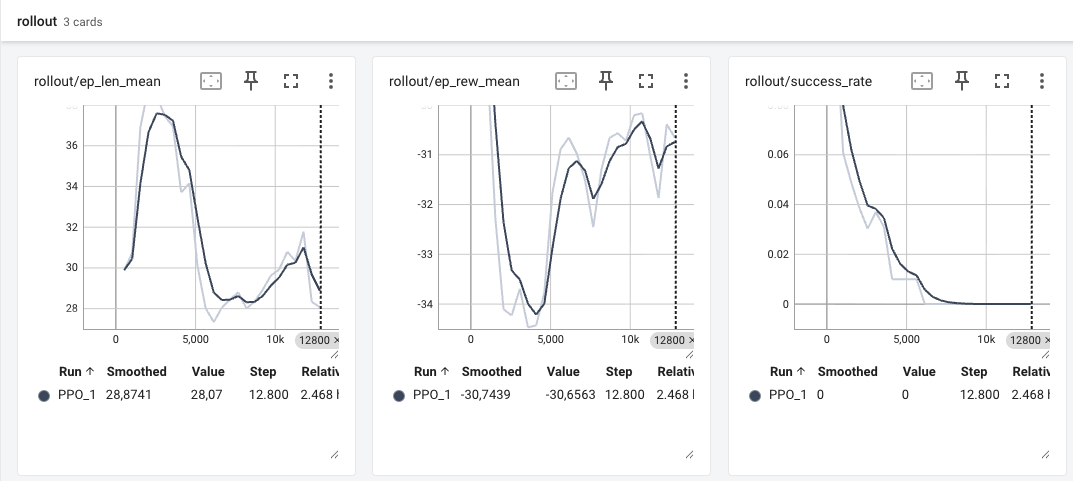
\includegraphics[width=0.95\textwidth]{images/tensorboard_exp010_rollout.png}
\caption{Métricas de \emph{rollout} de TensorBoard para Exp010. La tasa de éxito
desciende hasta cero y la recompensa media no muestra una tendencia sostenida de
mejora, por lo que la figura debe interpretarse como evidencia de diagnóstico y
no como demostración de aprendizaje estable.}
\label{fig:anexos:tensorboard_exp010_rollout}
\end{figure}

\begin{figure}[H]
\centering
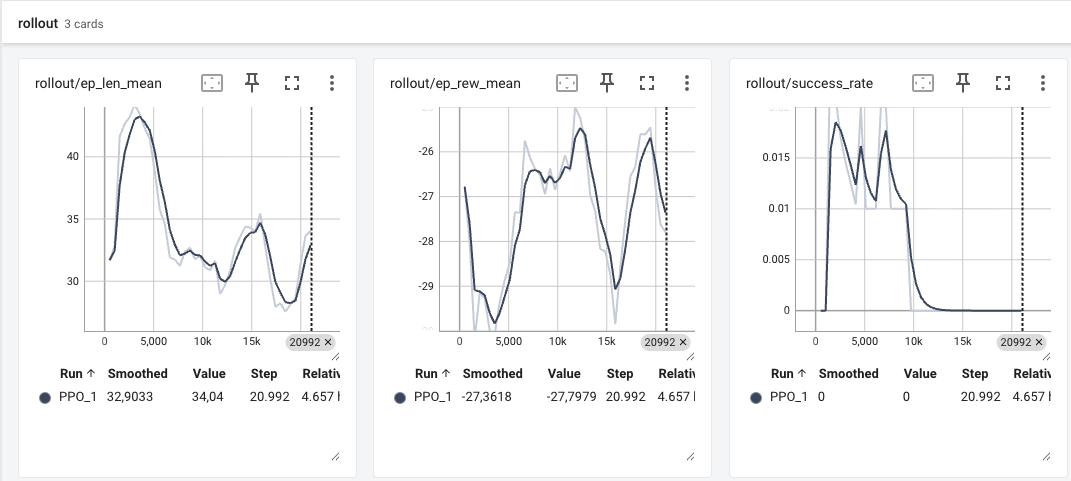
\includegraphics[width=0.95\textwidth]{images/tensorboard_exp011_rollout.png}
\caption{Métricas de \emph{rollout} de TensorBoard para Exp011. Aunque la
configuración reduce la saturación inicial y mejora parcialmente la recompensa
media frente a Exp010, la tasa de éxito vuelve a cero y las terminaciones por
límites o baja altitud siguen dominando el entrenamiento.}
\label{fig:anexos:tensorboard_exp011_rollout}
\end{figure}

\begin{figure}[H]
\centering
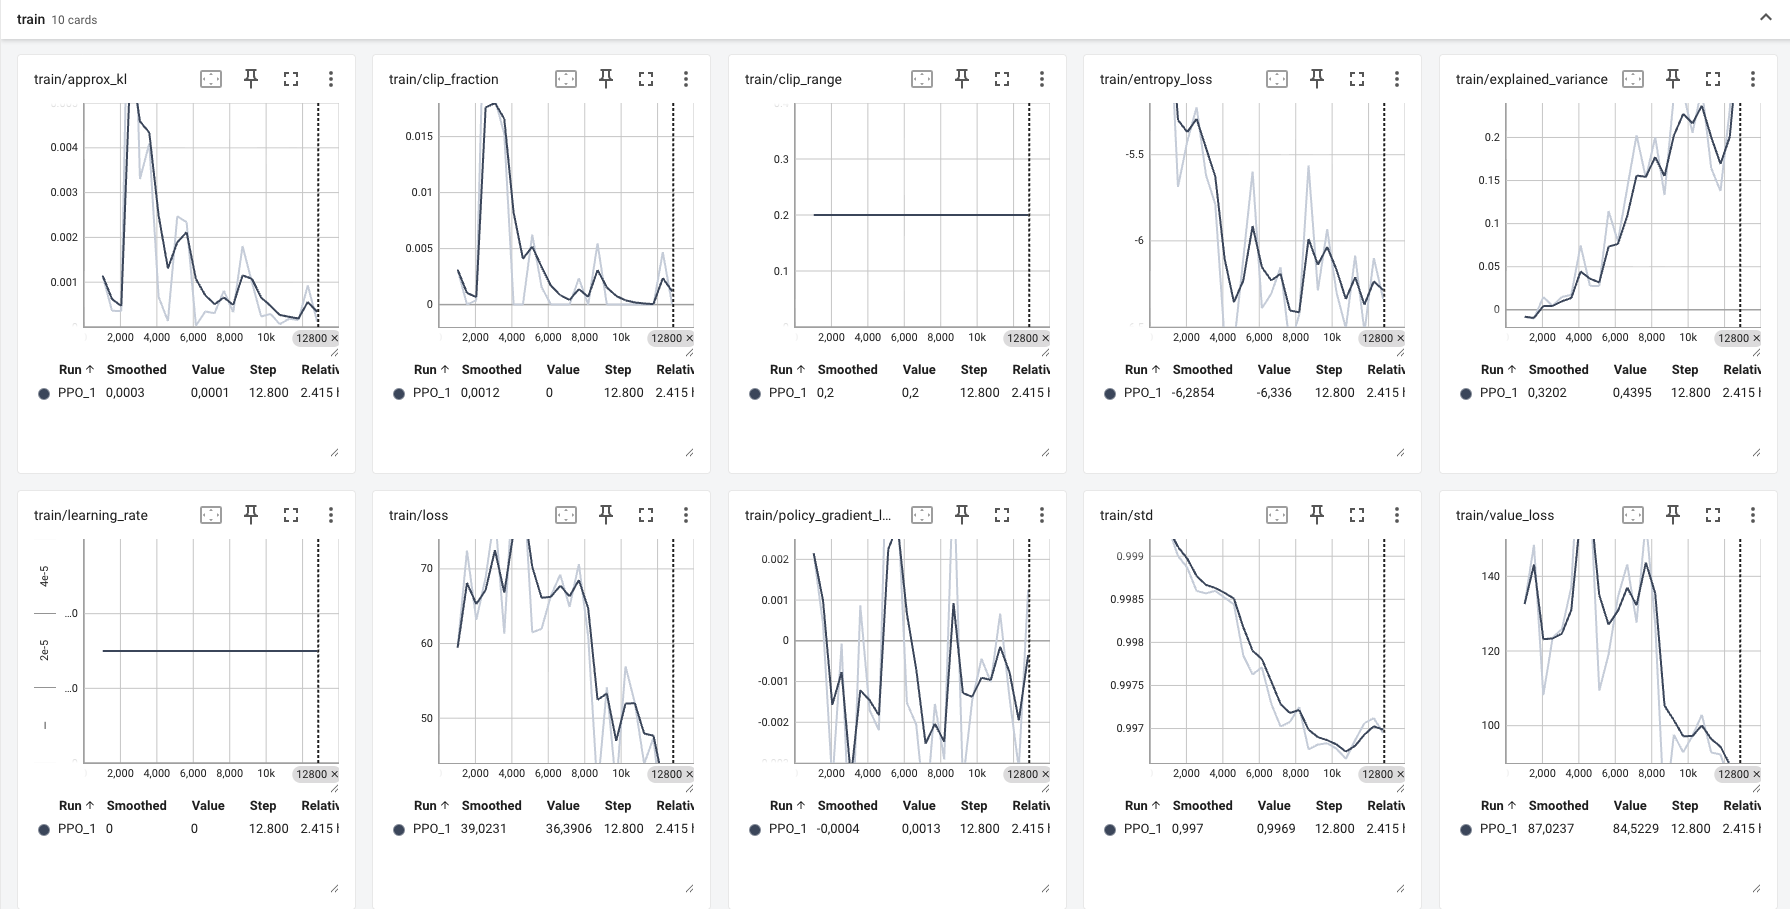
\includegraphics[width=0.95\textwidth]{images/tensorboard_exp010_train.png}
\caption{Métricas internas de PPO para Exp010. Los indicadores de entrenamiento
se mantienen en rangos razonables para una ejecución estable de PPO, pero esto no
implica éxito de la tarea cuando las métricas de episodio muestran predominio de
terminaciones no deseadas.}
\label{fig:anexos:tensorboard_exp010_train}
\end{figure}

\begin{figure}[H]
\centering
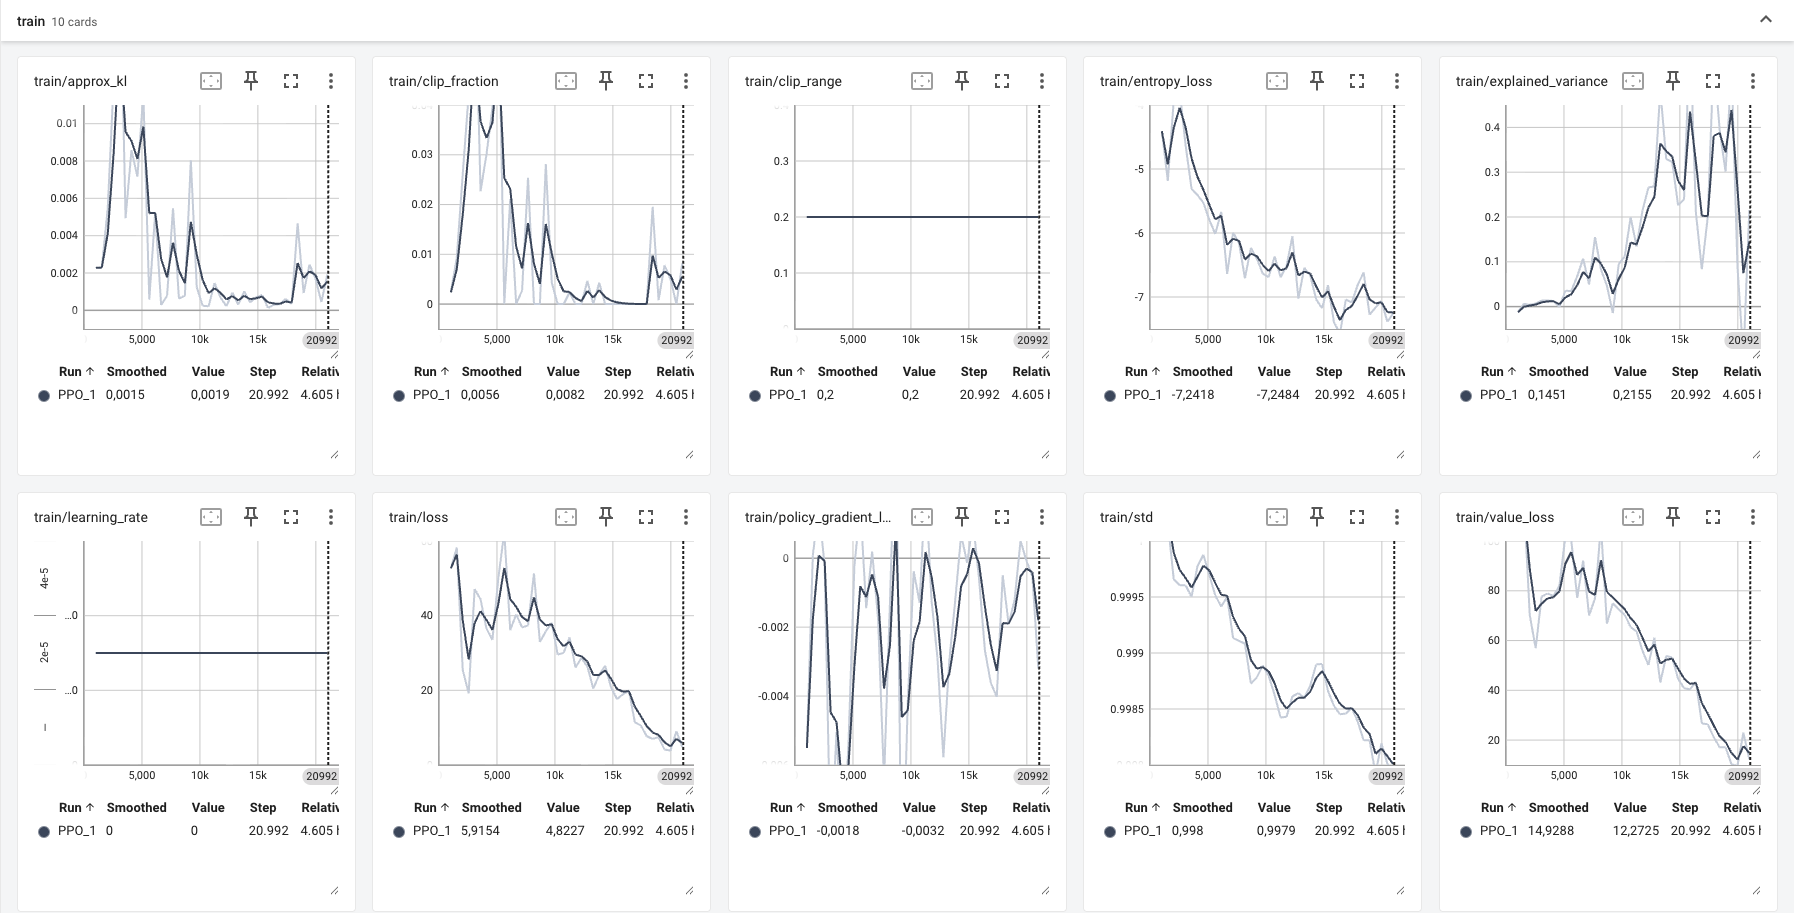
\includegraphics[width=0.95\textwidth]{images/tensorboard_exp011_train.png}
\caption{Métricas internas de PPO para Exp011. La evolución de pérdidas,
entropía y varianza explicada se utiliza como apoyo técnico, mientras que la
interpretación principal del experimento se obtiene de las métricas de
\emph{rollout} y de los monitores de episodio.}
\label{fig:anexos:tensorboard_exp011_train}
\end{figure}

\section{Declaración de uso de herramientas de inteligencia artificial} \label{sct:anexos:uso_ia}

Durante la realización del presente trabajo se han empleado herramientas de
inteligencia artificial generativa como apoyo a tareas de programación,
diagnóstico, organización de resultados y organización en la redacción. En particular, se ha
utilizado OpenAI Codex en el entorno de desarrollo para asistencia sobre código,
inspección del repositorio, generación de propuestas de modificación, revisión de
errores y apoyo a la edición de la memoria \cite{openai2026codex}. También se ha
utilizado ChatGPT como asistente conversacional para estructurar explicaciones,
revisar redacción y sintetizar criterios de presentación académica
\cite{openai2026chatgpt}.

El uso de estas herramientas no sustituye la autoría ni la responsabilidad
académica del trabajo. Las decisiones de diseño, la interpretación de resultados,
la selección de experimentos y la aceptación final de cambios se han revisado a
partir del repositorio, de las trazas de ejecución, de los ficheros de
configuración y de los logs experimentales. Las
respuestas generadas por IA se han tratado como propuestas de trabajo que debían
ser verificadas, corregidas o descartadas antes de incorporarse al documento o al
código.

\begin{table}[H]
\centering
\small
\setlength{\tabcolsep}{4pt}
\renewcommand{\arraystretch}{1.15}
\begin{tabular}{p{0.22\textwidth} p{0.32\textwidth} p{0.34\textwidth}}
\hline
\textbf{Herramienta} & \textbf{Tareas asistidas} & \textbf{Validación aplicada} \\
\hline
OpenAI Codex & Inspección del repositorio, edición de LaTeX, revisión de errores de compilación y apoyo a cambios de código. & Revisión manual de los diffs, compilación de LaTeX y contraste con el repositorio.\\
ChatGPT & Estructuración de explicaciones, síntesis de resultados y apoyo a redacción académica. & Revisión del texto, eliminación de afirmaciones no respaldadas y contraste con evidencias experimentales. \\
\hline
\end{tabular}
\caption{Resumen del uso de herramientas de inteligencia artificial generativa.}
\label{tab:anexos:uso_ia}
\end{table}

Entre los prompts más relevantes se encuentran los dirigidos a analizar 
el estado real del repositorio y del registro experimental, a
identificar diferencias entre resultados de entrenamiento y resultados de
infraestructura. Por otra parte para revisar la compilación LaTeX y para organizar la 
incorporación de figuras y tablas. 

No se han utilizado las herramientas de inteligencia artificial como fuente
bibliográfica primaria sobre aprendizaje por refuerzo, ROS 2, Aerostack2 o
Stable-Baselines3. Las afirmaciones técnicas del cuerpo de la memoria se apoyan
en referencias bibliográficas, documentación técnica, código implementado y
evidencia experimental. Cuando se ha incorporado texto redactado con apoyo de IA,
este se ha revisado y adaptado para mantener el tono académico, la precisión
terminológica y la coherencia con los resultados disponibles.
